\begin{frame}
	\frametitle{Kreisläufe, Resbudget und Kipppunkte - Zusammenfassung}
	\begin{columns}
		\column{0.3\linewidth}
			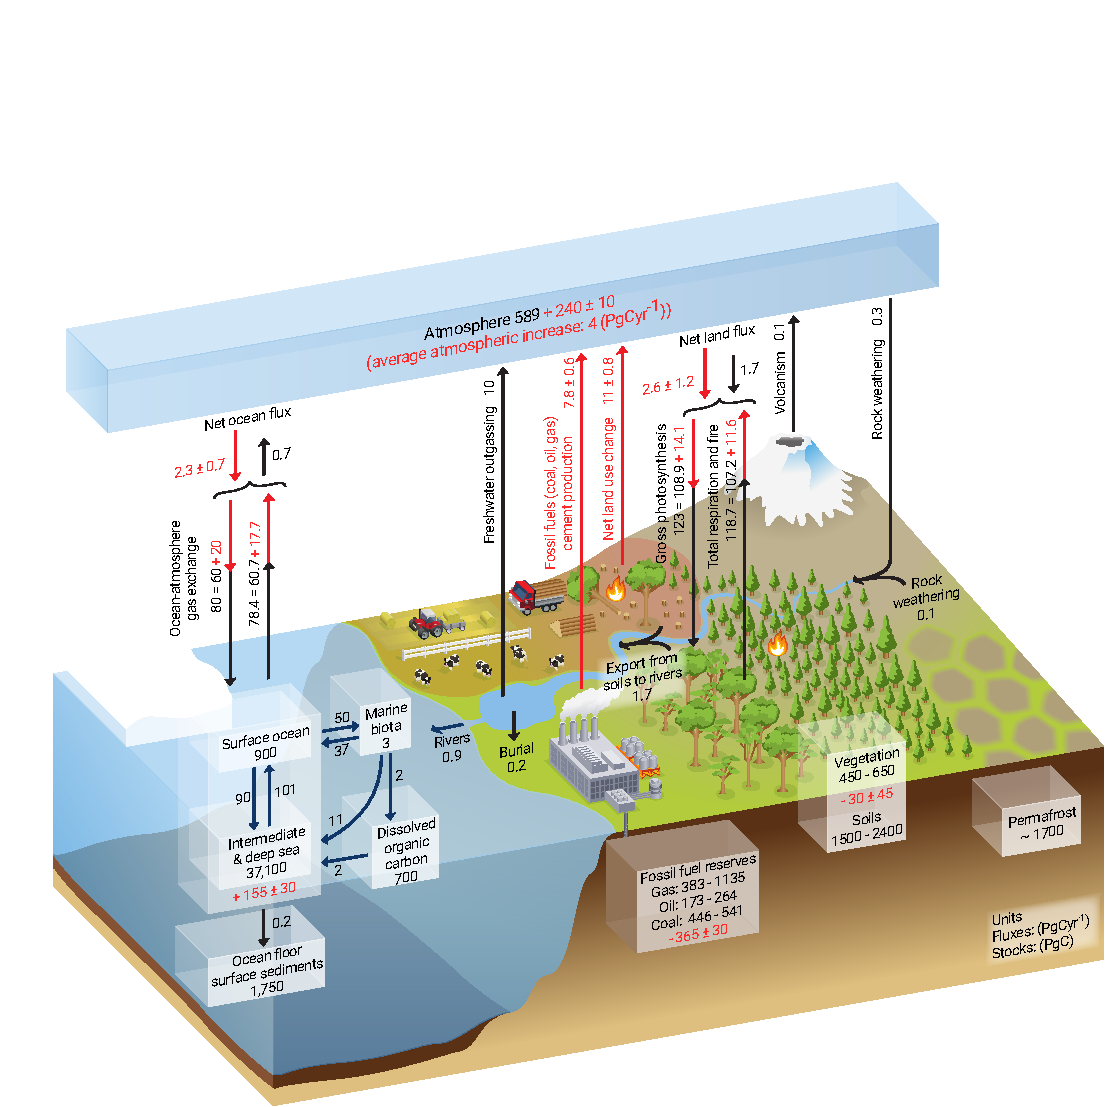
\includegraphics[trim={1cm 0cm 0cm 3cm}, clip, width=0.8\linewidth]{bilder/kohlenstoff/carbon_cycle_industrial-ocean.pdf}
		\column{0.7\linewidth}
			\begin{itemize}
				\item Im Erdsystem werden große Stoffmengen umgesetzt.
				\item Der Mensch hat einen deutlichen Einfluss und erhöht den Kohlenstoffgehalt in der Atmosphäre jährlich um etwa \SI{4}{\GtCO}.
			\end{itemize}
	\end{columns}
	\begin{columns}
		\column{0.7\linewidth}
			\begin{itemize}
				\item Das CO$_2$-Restbudget zum erreichen des \SI{1.5}{\degreeCelsius} Ziels lässt sich mit Hilfe vieler Klimamodelle mit Eintrittswahrscheinlichkeiten abschätzen.
				\item Bei gleichbleibender Emission sind die Restbudgets in 8,5 bzw. 11,8 Jahren aufgebraucht.
			\end{itemize}
		\column{0.3\linewidth}
			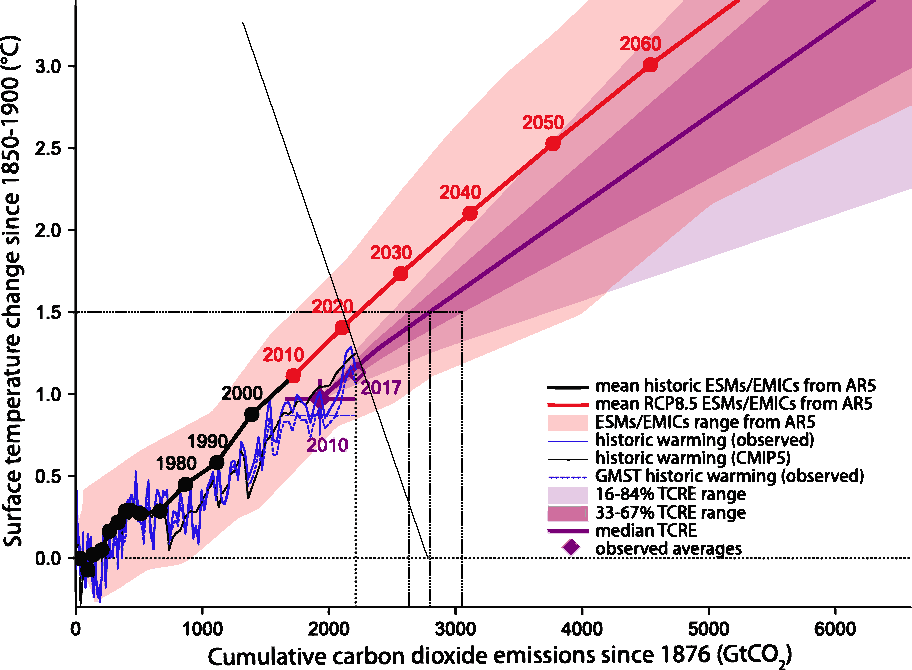
\includegraphics[width=0.9\linewidth]{bilder/cumulative_co2/cumulative_co2-4.pdf}
	\end{columns}
	\begin{columns}
		\column{0.3\linewidth}
			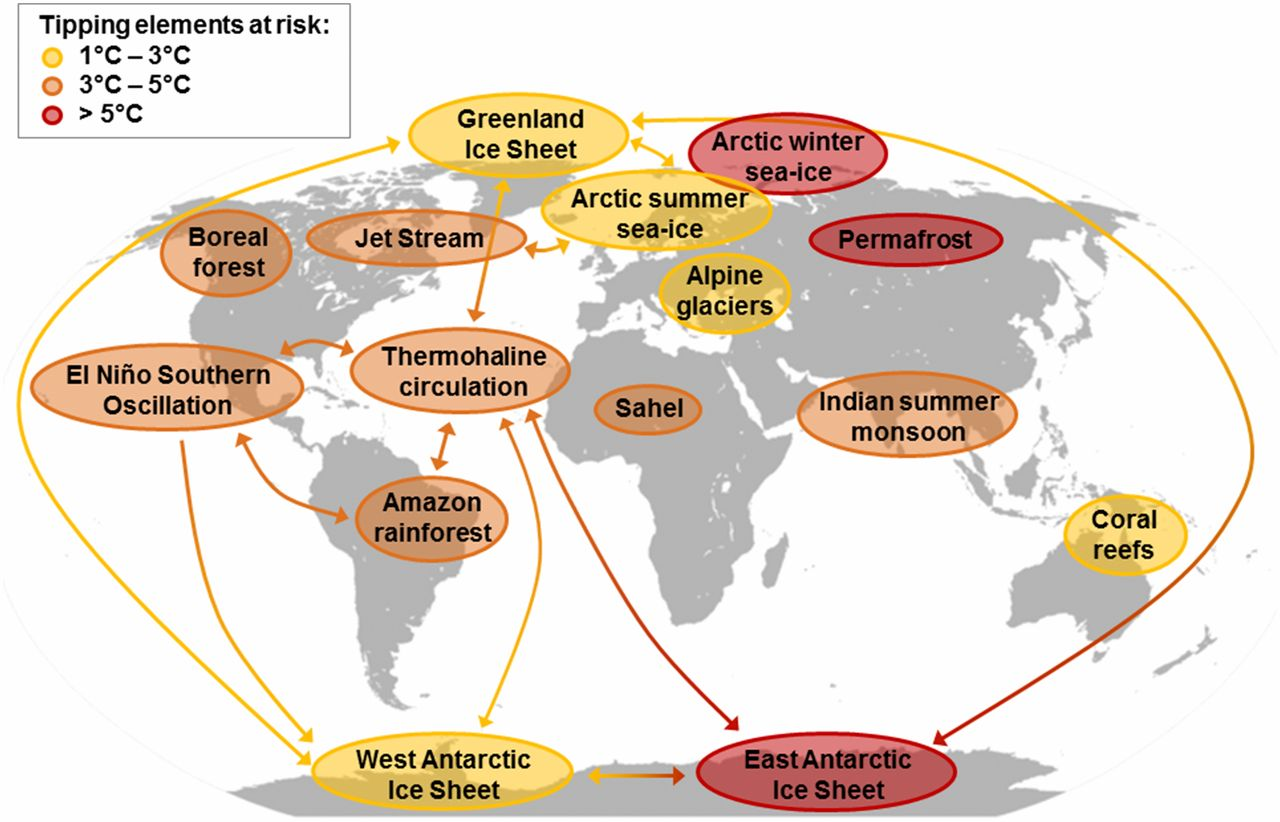
\includegraphics[width=0.9\linewidth]{bilder/kipppunkte/tipping_elements}
		\column{0.7\linewidth}
			\begin{itemize}
				\item Komplexe Systeme können mehrere Gleichgewichtszustände haben, die bei groß genügender Änderung in einen neuen dauerhaften Zustand übergehen können.
				\item Kipppunkte sind sich selbstverstärkende Effekte und sind ab einem gewissen Punkt kaum noch aufhaltbar.
			\end{itemize}
	\end{columns}
\end{frame}
